\section{Background and Related Work}
\label{sec:background}

\subsection{OIDC Services}
\label{subsec:OIDC}
OIDC is one of the most popular SSO protocols. It supports different login flows: implicit flow, authorization code flow, and hybrid flow (a mix of the other two). These flows differ in the steps for requesting, receiving and forwarding tokens, but have common security requirements for identity tokens.
We present our designs in the implicit flow and discuss the support for the authorization code flow in Section \ref{sec:discussion}.

Users and RPs register at an OIDC IdP with their identities
and other information such as user credentials %(e.g., passwords)
and RP endpoints. %(i.e., the URLs to receive tokens).
As shown in Figure \ref{fig:OpenID}, on receiving a login request, an RP constructs an identity-token request with its identity and the scope of requested user attributes.
This request is posted (or redirected) to the IdP.
After authenticating the user, the IdP issues an identity token that encloses the (pseudo-)identities of the user and the target RP, the requested attributes, a validity period, etc. The user then forwards the identity token to the RP's endpoint. The RP verifies the token and allows the holder to log in as the user (pseudo-)identity enclosed.

\begin{figure}[b]
  \centering
  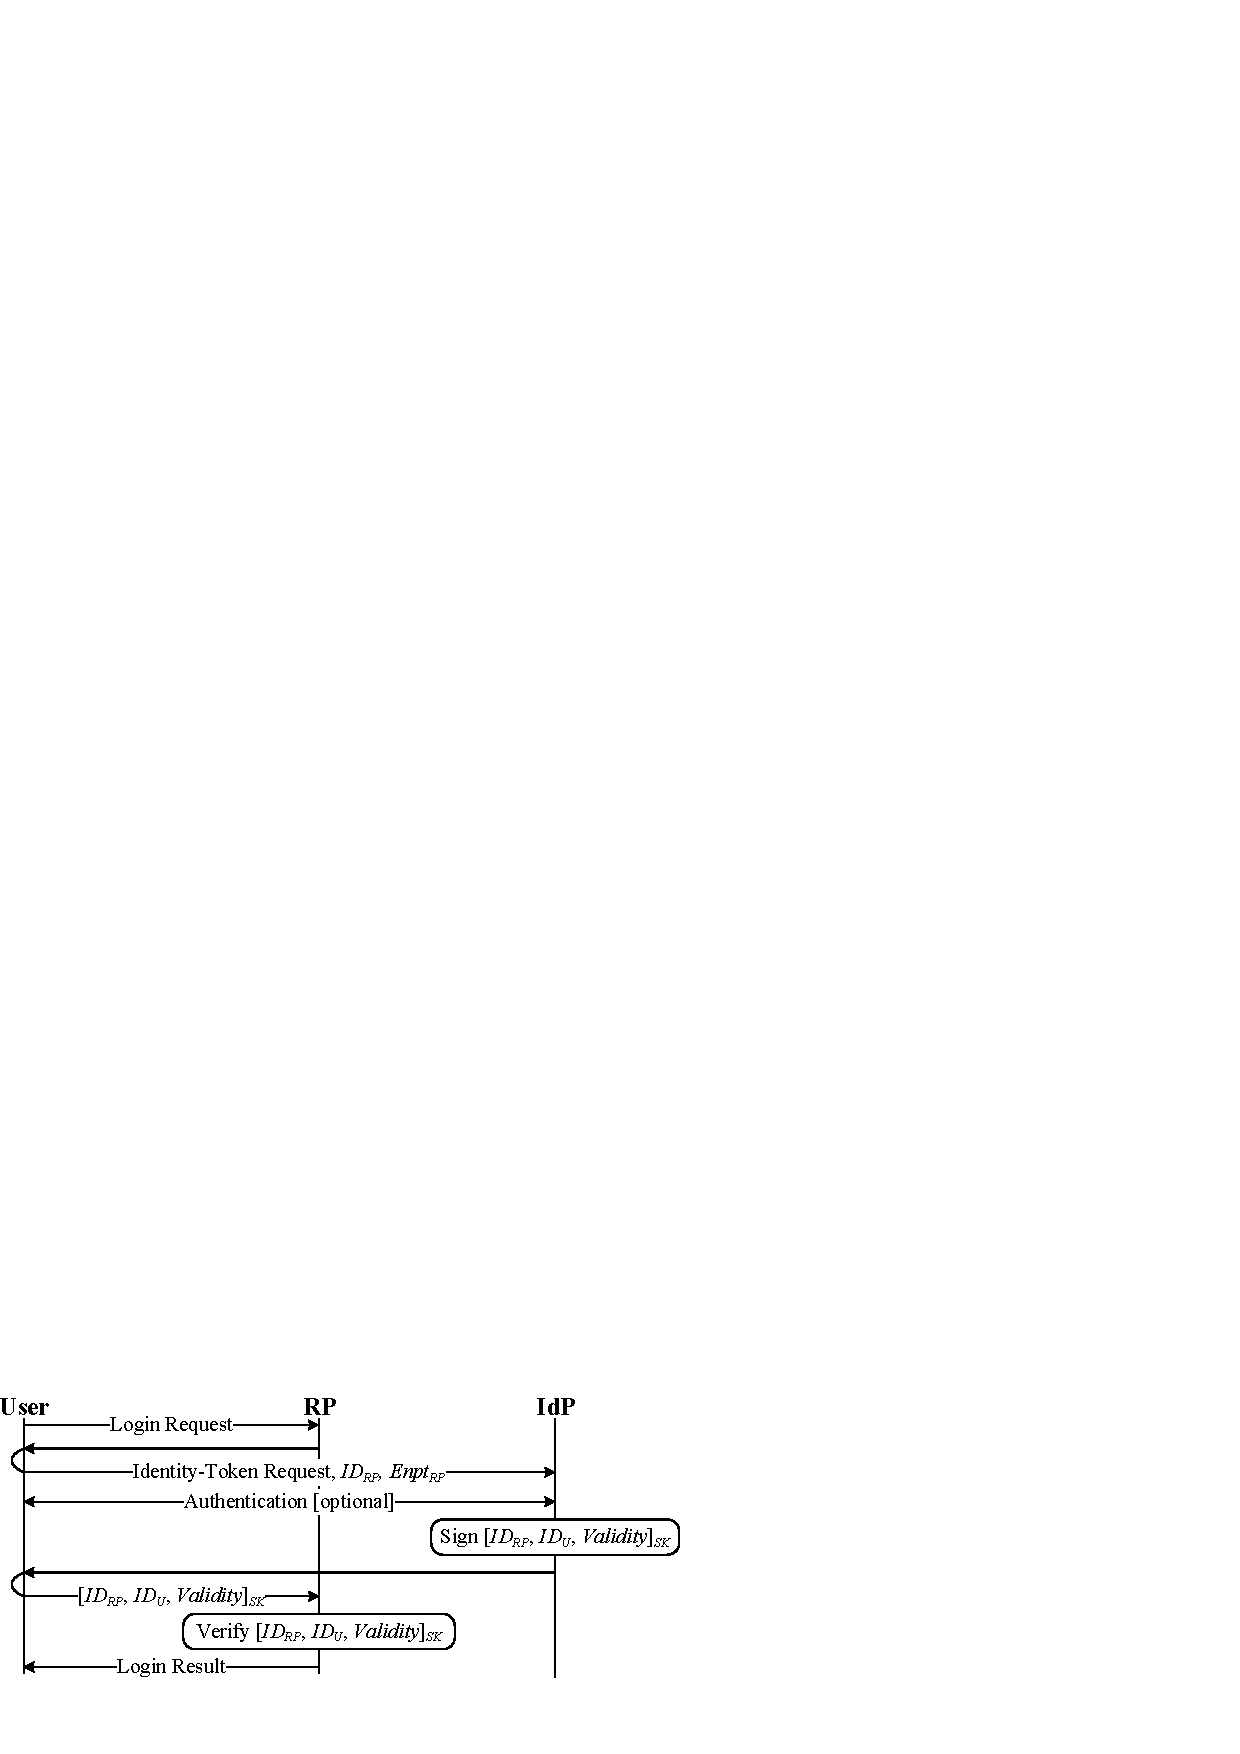
\includegraphics[width=1.0\linewidth]{fig/OIDC.pdf}
  \caption{The implicit SSO login flow of OIDC}
  \label{fig:OpenID}
\end{figure}

\begin{table*}[tb]
\small
    \caption{Privacy-preserving solutions of SSO and identity federation}
    \centering
    \begin{tabular}{|c|c|c|c|c|c|c|c|}
  \hline
  & \multirow{3}*{\textbf{Solution}} &
  \multicolumn{3}{c|}{\textbf{Service Feature}$^{\dag}$} & \multicolumn{2}{c|}{\textbf{Privacy Threat}$^{\sharp}$} & \textbf{Extra} \\ \cline{3-7}
  & & User Authentication & User Identification & IdP-confirmed & IdP-based & RP-based & \textbf{Trusted} \\
  & & Only to the IdP & at Each RP & Attribute Provision & Login Tracing & Identity Linkage & {\textbf{Server}$^{\ddag}$} \\\hline
  \multirow{5}*{SSO} & OIDC w/ PPID \cite{NIST2017draft} & $\CIRCLE$ & $\CIRCLE$ & $\CIRCLE$ & $\Circle$ & $\CIRCLE$ & $\CIRCLE$ \\ \cline{2-8}
   & BrowserID \cite{BrowserID} & $\CIRCLE$ & $\CIRCLE$ & $\Circle$ & $\CIRCLE$ & $\Circle$ & $\CIRCLE$ \\ \cline{2-8}
   & SPRESSO \cite{SPRESSO} & $\CIRCLE$ & $\CIRCLE$ & $\Circle$ & $\CIRCLE$ & $\Circle$ & $\Circle$$^1$ \\ \cline{2-8}
   & POIDC \cite{POIDC,save-flow} & $\CIRCLE$ & $\CIRCLE$ & $\CIRCLE$ & $\CIRCLE$ & $\Circle$ & $\CIRCLE$ \\ \cline{2-8}
   & MISO \cite{miso} & $\CIRCLE$ & $\CIRCLE$ & $\CIRCLE$ & $\CIRCLE$ & $\CIRCLE$ & $\Circle$ \\ \hline 
  \multirow{5}*{\makecell{Identity\\Federation}} & PRIMA \cite{prima} & $\Circle$ & $\CIRCLE$ & $\CIRCLE$ & $\CIRCLE$ & $\Circle$ & $\CIRCLE$ \\ \cline{2-8}
   & PseudoID \cite{PseudoID} & $\Circle$ & $\CIRCLE$ & $\Circle$ & $\CIRCLE$ & $\CIRCLE$ & $\Circle$ \\ \cline{2-8}
   & Opaak \cite{Opaak} & $\Circle$ & $\LEFTcircle$$^2$ & $\Circle$ & $\CIRCLE$ & $\CIRCLE$ & $\CIRCLE$ \\ \cline{2-8}
 % U-Prove \cite{uprov} & $\CIRCLE$ & $\Circle$ & $\LEFTcircle$$^6$ & $\CIRCLE$ & $\CIRCLE$ & $\CIRCLE$ \\ \hline
 % UnlimitID \cite{UnlimitID} & $\CIRCLE$ & $\Circle$ & $\CIRCLE$ & $\CIRCLE$ & $\CIRCLE$ & $\CIRCLE$ \\ \hline
 % EL PASSO \cite{ELPASSO} & $\CIRCLE$ & $\Circle$ & $\CIRCLE$ & $\CIRCLE$ & $\CIRCLE$ & $\CIRCLE$ \\ \hline
   & PP-IDF \cite{ELPASSO,uprov,UnlimitID} & $\Circle$ & $\CIRCLE$ & $\CIRCLE$$^3$ & $\CIRCLE$ & $\CIRCLE$ & $\CIRCLE$ \\ \cline{2-8}
   & Fabric Idemix \cite{hyperledge-idemix} & $\Circle$ & $\LEFTcircle$$^4$ & $\CIRCLE$ & $\CIRCLE$ & $\CIRCLE$ & $\CIRCLE$ \\ \hline
 % PrivacyPass \cite{privacypass,trusttoken} & $\Circle$ & $\Circle$ & $\Circle$ & $\CIRCLE$ & $\CIRCLE$ & $\Circle$ \\ \hline
  SSO & \usso & $\CIRCLE$ & $\CIRCLE$ & $\CIRCLE$ & $\CIRCLE$ & $\CIRCLE$ & $\CIRCLE$ \\ \hline
\end{tabular}
    \label{tbl:comparison-protocol}
{\flushleft
${\dag}$. \textbf{Service Feature}: $\CIRCLE$ supported, $\Circle$ unsupported, $\LEFTcircle$ partially supported. \ \ \ \ \ \ \ \ \ \ \ \ 
${\sharp}$. \textbf{Privacy Threat}: $\CIRCLE$ prevented, $\Circle$ not prevented.

${\ddag}$. \textbf{Extra Trusted Server}: $\CIRCLE$ without, $\Circle$ required.

1. SPRESSO assumes a \emph{malicious} IdP (but honest IdPs in others), and a forwarder server is trusted to decrypt the RP identity and forward tokens to the RP.

2. Opaak supports two exclusive pseudonym options: (\emph{a}) linkable within an RP but unlinkable across multiple RPs and (\emph{b}) unlinkable for any pair of actions.

3. Different from \cite{ELPASSO,UnlimitID}, a credential in U-Prove \cite{uprov} may contain some attributes that are \emph{invisible} to the IdP, in addition to the ones confirmed by the IdP.

4. In the original design of Idemix \cite{idemix}, every user logs into an RP with a unique account, but Fabric Idemix \cite{hyperledge-idemix} implements completely-anonymous services.}
\end{table*}

User operations in OIDC are conducted by a user agent (or browser typically).
To process tokens retrieved from the IdP, which is carried with a URL following the fragment identifier \texttt{\#} instead of \texttt{?} due to security considerations \cite{de2014oauth},
%To process responses from an IdP and forward tokens to the target RP correctly,
    a COTS browser needs to download a web script from the visited RP,
        called the \emph{user-r} script.
Further,
    another \emph{user-i} script downloaded from the IdP server,
    is recommended to provide an in-context user experience  \cite{dimvaLiM16,GoogleIdIntegrate,uber}, which is called \emph{pop-up UX},
    for the user's attribute authorization.
Then, two scripts are responsible for communicating with the respective origin servers (e.g., token requesting, receiving and forwarding) and also the cross-origin
communications using the \verb+postMessage+ HTML5 API within a browser.
Alternatively, if a browser works as the user agent with \emph{only} the user-r script,
        user attributes are authorized in the redirected IdP window.
    This is called \emph{redirect UX}.

The following features are desired in SSO services and supported by OIDC and other popular SSO protocols \cite{NIST2017draft, OpenIDConnect,rfc6749, SAML, SAMLIdentifier}.

\noindent\textbf{User authentication only to the IdP.}
RPs only verify the identity tokens issued by an IdP, and the authentication between a user and the IdP is conducted \emph{independently} of the steps where identity tokens are generated.
This offers advantages. First, the IdP authenticates users by any appropriate means such as passwords, one-time passwords, or multi-factor authentication (MFA).
Meanwhile, a user only maintains her credential for the IdP. If it is lost or leaked, the user needs to renew it only at the IdP.

\noindent \textbf{User identification at each RP.}
An RP recognizes each user by an identity (or account) \emph{unique} within the RP to provide customized services across multiple logins.
Such non-anonymous SSO systems are more desirable in various applications than anonymous services.

\noindent\textbf{IdP-confirmed attribute provision.}
An IdP may enclose also user attributes in identity tokens along with user (pseudo-)identities \cite{OpenIDConnect,rfc6749}.
A user maintains her attributes at the trusted IdP,
which provides only pre-selected ones to RPs
    or obtains the user's authorization before enclosing attributes.

\subsection{Privacy-Preserving Solutions for SSO and Identity Federation}
\label{subsec-solutions}


SSO allows a user to log into an RP, without by herself maintaining an account at the RP or holding a long-term secret verified by the RP,
so that SSO services are accessible from COTS browsers.
On the contrary, identity federation enables a user registered at a trusted IdP to be accepted by other parties, potentially with different accounts,
but extra \emph{authentication operations between the user and RPs} are involved, so plug-ins or extensions are needed to access such services from a browser.
Thus, although the term ``single sign-on (SSO)'' was used in some schemes \cite{PseudoID, Opaak, ELPASSO, WangWS13, HanCSTW18, HanCSTWW20}, this paper refers to them as \emph{identity federation} to emphasize this difference.

Table \ref{tbl:comparison-protocol} compares privacy-preserving schemes of SSO and identity federation,
        by analyzing whether a service feature is supported
                and whether a privacy threat is prevented or not.
This table also shows whether an extra trusted server is required, in addition to the IdP.
Among them only \usso\ satisfies all desirable properties.

%Privacy-preserving SSO is expected to offer the desirable features listed in Section \ref{subsec:OIDC}, while addressing privacy threats.
%Privacy-preserving identity federation offers more privacy protections, but brings extra complexity to users as described above.


\noindent\textbf{Privacy-preserving SSO.}
Some schemes \cite{BrowserID, SPRESSO, NIST2017draft} prevent either IdP-based login tracing or RP-based identity linkage, but not both.
First of all, pairwise pseudonymous identifiers (PPIDs) are specified \cite{OpenIDConnect, SAMLIdentifier} and recommended \cite{NIST2017draft} in OIDC to protect user privacy against colluding RPs.
An IdP assigns a unique PPID for a user to log into some RP and encloses it in identity tokens, so colluding RPs cannot link the user.
It does not prevent IdP-based login tracing because the IdP needs the RP's identity to assign PPIDs.


Other privacy-preserving SSO schemes prevent IdP-based login tracing but leave users vulnerable to RP-based identity linkage, due to the globally-unique user identities enclosed in identity tokens.
For example, in BrowserID \cite{BrowserID} 
after authenticating a user,
    an IdP %(called the primary identity authority in BrowserID)
issues a ``user certificate'' binding the user's identity but no attribute to an \emph{ephemeral} public key.
The user then uses the private key to sign a subsidiary ``identity assertion'' that binds the target RP's identity and sends both of them to the RP.
In SPRESSO an RP creates a one-time tag (or pseudo-identity) for each login \cite{SPRESSO}, 
 or a user sends an identity-token request with a hash commitment on the target RP's identity in POIDC \cite{POIDC,save-flow},
        which are enclosed in identity tokens along with the user's unique identity.
As in SPRESSO the IdP is assumed to be malicious, there is no IdP-confirmed attribute provision.
Besides, a variation of POIDC \cite{POIDC} proposes to also hide a user's identity in the commitment and prove this to the IdP in zero-knowledge,
        but it takes seconds to generate such a zero-knowledge proof (ZKP) even for a powerful server \cite{ZKP-BINF,zkp-benchmark,ZKP-GPU},
        which is impracticable for a user agent in SSO systems.
% J. He, L. Lei \emph{et al}. \cite{ARPSSO} copied the identity transformations of \usso published in the preprint version \cite{uppresso-arxiv}, into a prime field $F_q$,\footnote{That is, $ID_U = u$, $ID_{RP} = h = g^r$, $PID_{RP} = h^t = g^{rt}$, $PID_U = h^{tu}=g^{rtu}$, and $Acct = h^u= g^{ru}$ in $F_q$ where $g$ is a generator. It seems that these identity transformations were called RP anonymization and user identity mix-up intentionally in ARPSSO \cite{ARPSSO}.} and attempted to implement \usso\ in the authorization code flow of OIDC using \emph{trusted} scripts without any extensions or plug-ins, which also follows the same principle as the \usso\ prototype does.

MISO \cite{miso} decouples the calculation of PPIDs from an honest IdP in OIDC,
 to \emph{an extra trusted mixer server} that calculates a user's PPID based on $ID_U$, $ID_{RP}$ and a secret after it receives the authenticated user's identity from the IdP.
MISO prevents both RP-based identity linkage for the RPs receives only PPIDs,
    and IdP-based login tracing for $ID_{RP}$ is disclosed to the mixer but not the IdP.
It protects a user's online profile against even collusive attacks by the IdP and RPs,
    but the mixer server could track a user's all login activities.

\noindent\textbf{Privacy-preserving identity federation.}
First of all, in these schemes \cite{prima,PseudoID,Opaak, ELPASSO,uprov,UnlimitID,hyperledge-idemix},
    additional authentication operations between the user and RPs are involved.

In PRIMA \cite{prima}, an IdP signs a credential
that binds user attributes and a verification key. Using the signing key, the user provides selected attributes to RPs. This verification key works as the user's identity and exposes her to RP-based identity linkage.
PseudoID \cite{PseudoID} introduces another trusted server in addition to the IdP,
 to blindly sign \cite{blind-sign}
an access token that binds a user secret, a pseudonym but no other user attributes.
The user then unblinds this token,
    authenticates herself to an RP using the secret,
        and log into it.

Several schemes \cite{Opaak, hyperledge-idemix, uprov, UnlimitID, ELPASSO} are designed based on anonymous credentials \cite{anon-credential-2001, idemix, anon-credential}.
For instance, the IdP signs anonymous credentials in Opaak \cite{Opaak}, UnlimitID \cite{UnlimitID}, U-Prove \cite{uprov}, and EL PASSO \cite{ELPASSO}, each of which binds a long-term user secret. %, with which users can authenticate to an RP.
Then a user proves ownership of the anonymous credentials using her secret,
     and discloses IdP-confirmed attributes in the credentials in most schemes except Opaak.
Similarly, Fabric \cite{hyperledge-idemix} integrates Idemix anonymous credentials \cite{idemix} for completely-unlinkable pseudonyms and IdP-confirmed attribute provision.


Some privacy-preserving identity federation solutions \cite{PseudoID,Opaak,ELPASSO,uprov,UnlimitID,hyperledge-idemix} prevent both IdP-based login tracing and RP-based identity linkage, for (\emph{a}) the RP's identity is not enclosed in the anonymous credentials and (\emph{b}) the user selects different pseudonyms to visit different RPs.
They even protect user privacy against collusive attacks by the IdP and RPs, as these pseudonyms cannot be linked through anonymous credentials \cite{anon-credential-2001, idemix, anon-credential} when the ownership of these credentials is proved to colluding RPs. % using a user secret.
However, this protection brings extra complexity to users,
        and such services cannot be accessed from COTS browsers.
In Section \ref{sec:discussion}
we particularly discuss the collusion of the IdP and RPs in privacy-preserving SSO.


\noindent\textbf{Anonymous identity federation.}
Such approaches offer the strongest privacy,
    where a user visits RPs with pseudonyms that cannot be used to link any two actions.
Anonymous identity federation was formalized \cite{WangWS13} and implemented using cryptographic primitives such as group signature and ZKP \cite{WangWS13, HanCSTWW20, HanCSTW18}.
Extended designs including proxy re-verification \cite{HanCSTWW20}, designated verification \cite{HanCSTW18} and distributed IdP servers \cite{TSAPP}, are also considered. 

These completely-anonymous authentication services only work for special applications and do not support user identification at each RP, a common requirement in most applications.

